\chapter{Erstellung von Orthofotos der HSR}

%----------------------------------------------------------------------------------------

Die folgenden Kapitel beschreiben den Prozess, der nötig war um ein
georeferenziertes Orthofoto sowie ein georeferenziertes texturiertes
Oberflächenmodell der Hochschule für Technik in Rapperswil zu erzeugen.

%----------------------------------------------------------------------------------------

\section{Erfassung des HSR-Geländes mit Kamera-Drohne}

Auf die Erfassung von Luftbildern mithilfe eines Multikopters sind wir bereits
in \autoref{workflow:drone} eingegangen. Deshalb möchten wir hier lediglich die
Unterschiede zur 3D-Erfassung des Schloss Rapperswils hervorheben.

Im Gegensatz zur 3D-Erfassung geht es bei der Herstellung von Orthofotos nicht
primär um die dreidimensionale Form eines Objektes, sondern darum, möglichst
senkrechte und verzerrungsfreie Bilder zu erstellen.

\needspace{8\baselineskip}
Wir haben wiederum den Team BlackSheep Discovery Pro Quadrokopter mit Gimbal
verwendet, diesmal jedoch nicht mit der GoPro Kamera, sondern mit einer Sony
Alpha 5100 und einer verzerrungsfreien Brennweite.
\begin{figure}[H]
	\centering
	\includegraphics[width=\textwidth]{images/copter1.jpg}
	\caption{Der Team BlackSheep Discovery Pro Quadrokopter}
	\label{img:copter1}
\end{figure}

\needspace{8\baselineskip}
\noindent Die Kamera wurde mit dem Gimbal so positioniert, dass sie senkrecht
nach unten zeigt.
\begin{figure}[H]
	\centering
	\includegraphics[width=\textwidth]{images/copter3.jpg}
	\caption{Die Kamera-Aufhängung}
	\label{img:copter3}
\end{figure}

\needspace{8\baselineskip}
\noindent Während wir beim ersten Versuch ein Smartphone als GPS-Tracker auf dem
Quadrokopter befestigt hatten, verwendeten wir diesmal ein dediziertes
GPS-Tracking-Gerät, ein \textit{Navin
miniHomer}\footnote{\url{https://www.znex.de/de/minihomer/}}. Der Tracker wurde
so konfiguriert, dass er 10 mal pro Sekunde die Position und Ausrichtung
aufzeichnete.
\begin{figure}[H]
	\centering
	\includegraphics[width=\textwidth]{images/copter2.jpg}
	\caption{Deutlich sichtbar: Der gelbe GPS-Tracker}
	\label{img:copter2}
\end{figure}

\needspace{8\baselineskip}
\noindent Während 10 Minuten flogen wir nun auf einer Höhe zwischen 50m und 120m
über das HSR-Gelände, um Bildmaterial von jedem Gebäude zu erhalten.
\begin{figure}[H]
	\centering
	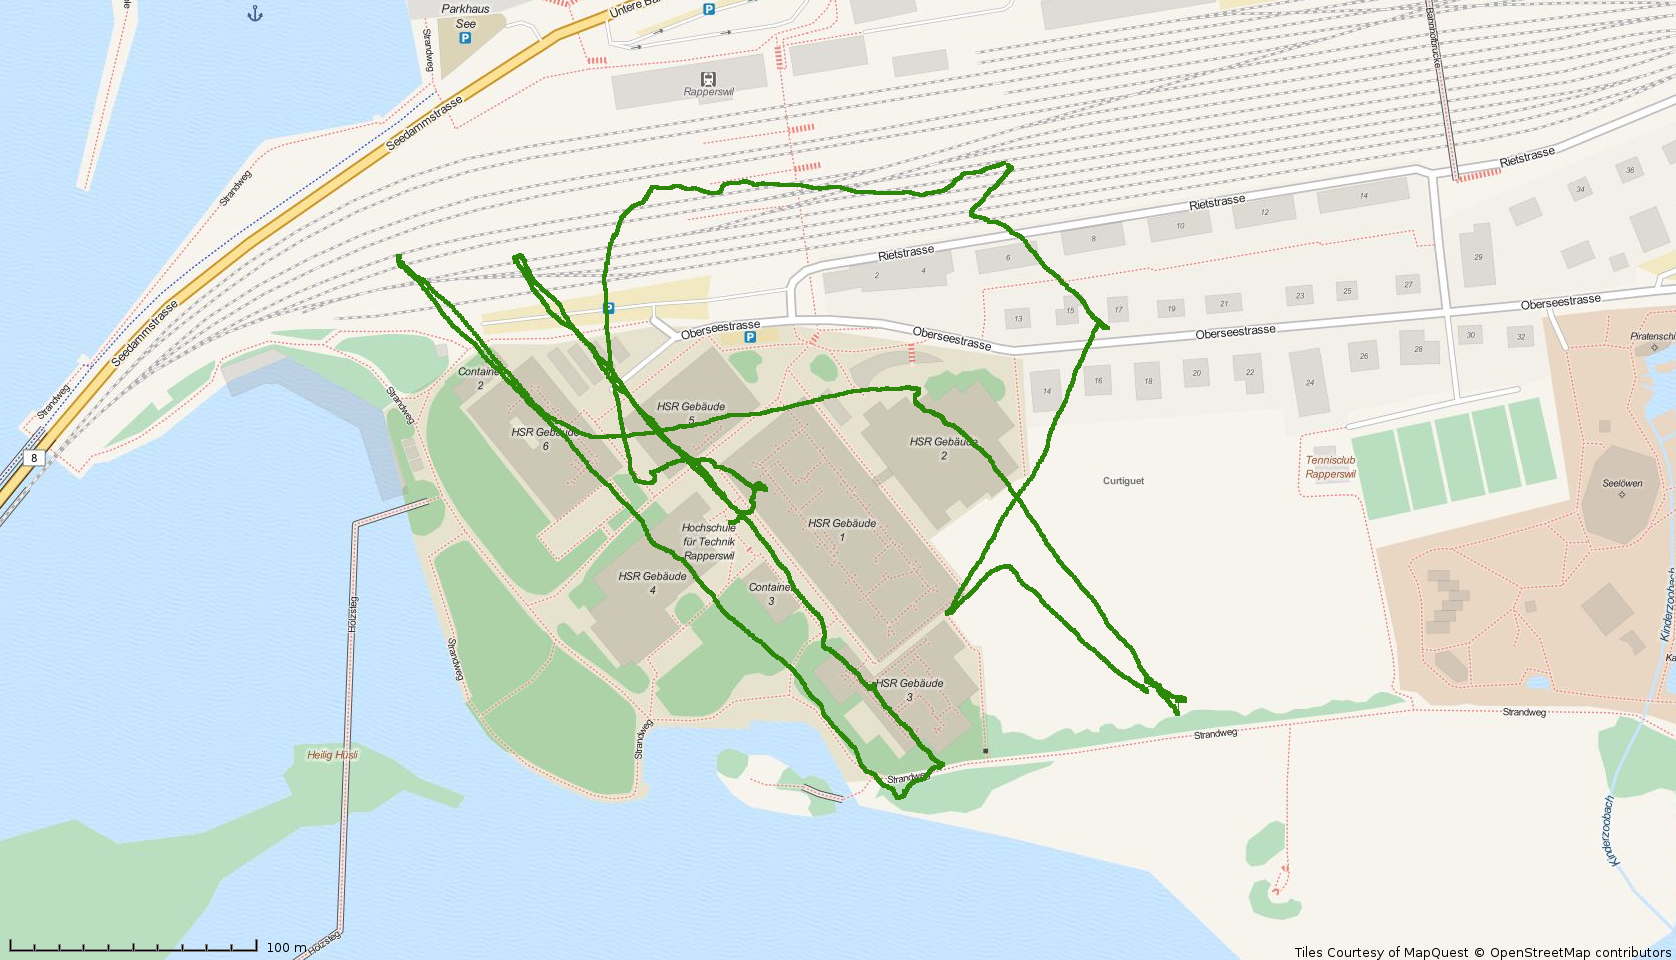
\includegraphics[width=\textwidth]{images/gpstrace_hsr_mapquest}
	\caption{GPS Trace des Quadkopters während der Erfassung.}
	\label{img:gpstrace_hsr_mapquest}
\end{figure}

%----------------------------------------------------------------------------------------

\section{Geocoding der Bilder}

Zurück zuhause sortierten wir die Bilder und löschten unbrauchbares
Bildmaterial. Anschliessend exportierten wir den GPS-Trace mithilfe von
\textit{GPSBabel}\footnote{\url{http://www.gpsbabel.org/}}:

\vspace{0.5\baselineskip}
\begin{minted}[bgcolor=tango-bg,frame=lines,framesep=2mm,samepage=true,fontsize=\footnotesize]{bash} 
gpsbabel -i skytraq -f /dev/ttyUSB0 -o gpx -F gps-recording.gpx
\end{minted}

Anschliessend muss diese Information in die Bild-Metadaten geschrieben werden.
Den Aufnahmezeitpunkt der Fotos kann mit dem Speicherzeitpunkt der
GPS-Messpunkte korreliert werden um so die entsprechende Position zu finden.

Um dies zu bewerkstelligen, gibt es verschiedene Tools. Wir haben
\textit{GPicSync}\footnote{\url{https://code.google.com/p/gpicsync/}} verwendet,
um die Geodaten im
IPTC-Format\footnote{\url{https://de.wikipedia.org/wiki/IPTC-IIM-Standard}} in
den Bildern zu speichern. Die verwendeten Einstellungen sind in
\autoref{img:gpicsync} ersichtlich.

\begin{figure}[h!]
	\centering
	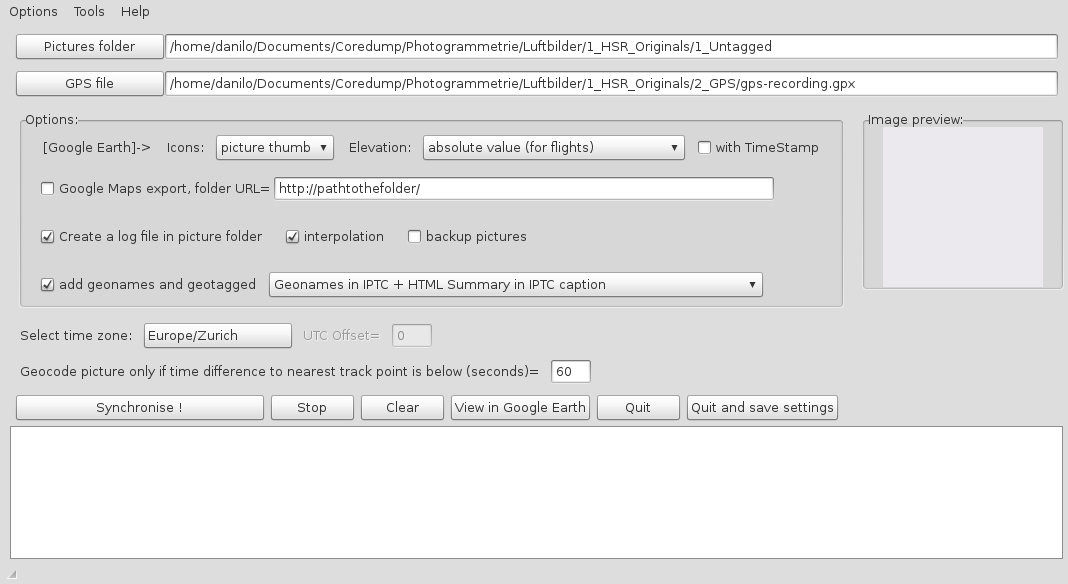
\includegraphics[width=\textwidth]{images/gpicsync}
	\caption{Einstellungen GPicSync}
	\label{img:gpicsync}
\end{figure}

Wichtig ist dabei vor allem ein möglicher Offset zwischen Kamera-Uhrzeit und
GPS-Uhrzeit. Man kann diese Abweichung relativ einfach berechnen, indem man ein
Foto des GPS-Geräts erstellt, auf welchem die genaue Uhrzeit ablesbar ist.
Der Offset ist die Differenz zwischen der Uhrzeit auf dem Foto und der Uhrzeit
in den Bild-Metadaten.

In \textit{GPicSync} kann der Offset über \texttt{Options > Local time
correction} konfiguriert werden, indem man die Uhrzeit beider Geräte eintippt.

%----------------------------------------------------------------------------------------

\section{Einführung OpenDroneMap}

%----------------------------------------------------------------------------------------

\section{Installation OpenDroneMap}

\subsection{Lokale Installation}
\subsection{Docker}

%----------------------------------------------------------------------------------------

\section{Generierung Orthofoto und Oberflächenmodell}

%----------------------------------------------------------------------------------------

\section{Resultate}
